\header{
    \headtitle{La rue Cuvier} \label{la-rue-cuvier}
    %
    
    \insertComment{Variante des carabins de Paris de la chanson marine toulonaise "En descendant la rue d'Alger".}{}
}

\enluminure{4}{\href{https://www.youtube.com/watch?v=QYoNqIWEPNc}{E}}n descendant la rue Cuvier \bissimple
\\Par une putain j'suis racolé \bissimple
\\ Elle me dit d'un air tendre
\\Eh bien!
\\De monter dans sa chambre
\\Et vous m'entendez bien?
\\Et nous t'entendons bien!
\\\\Moi qui suis d'l'université \bissimple
\\J'aime à savoir où j'mets les pieds \bissimple
\\J'achète une chandelle
\\Eh bien!
\\Pour monter chez la belle
\\Et vous m'entendez bien?
\\Et nous t'entendons bien!
\\\\Moi qui n'suis qu'un gros dégoûtant \bissimple
\\Je monte l'escalier en m'branlant \bissimple
\\En haut j'la carambole
\\Eh bien!
\\Elle avait la vérole
\\Et vous m'entendez bien?
\\Et nous t'entendons bien!
\\\\Quand la vérole fut attrapée \bissimple
\\A l'hôpital phallus t'aller \bissimple
\\L'hôpital maritime
\\Eh bien!
\\Me faire soigner la pine
\\Et vous m'entendez bien?
\\Et nous t'entendons bien!
\breakpage
Ils m'ont foutu pour me soigner \bissimple
\\4 Carabins 6 PCB \bissimple
\\Mais cette bande d'andouilles
\\Eh bien!
\\Ils m'ont coupé les couilles
\\Et vous m'entendez bien?
\\Et nous t'entendons bien!
\\\\\textit{Voix très aigue :}
\\Quand on a plus ni couilles, ni vit \bissimple
\\Rien ne vous plaît ni vous sourit \bissimple
\\On s'en va au bordel
\\Eh bien!
\\Faire minette aux maquerelles
\\Et vous m'entendez bien?
\\Et nous t'entendons bien!
\\\\\textit{Voix très grave :}
\\Depuis ce jour soir et matin \bissimple
\\Je maudis toutes les putains \bissimple
\\Car elles me rappellent
\\Eh bien!
\\Mes couilles qu'étaient si belles
\\Et qui marchaient si bien \}  ter
\begin{center}
   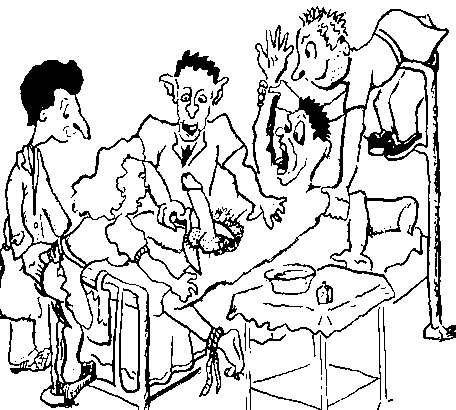
\includegraphics[width=0.7\textwidth]{images/cuvier.jpg}
 \end{center}

\breakpage